\documentclass{article}
\usepackage{pgfplots}
\pgfplotsset{compat=newest}

\begin{document}

\begin{figure}[h]
    \centering
    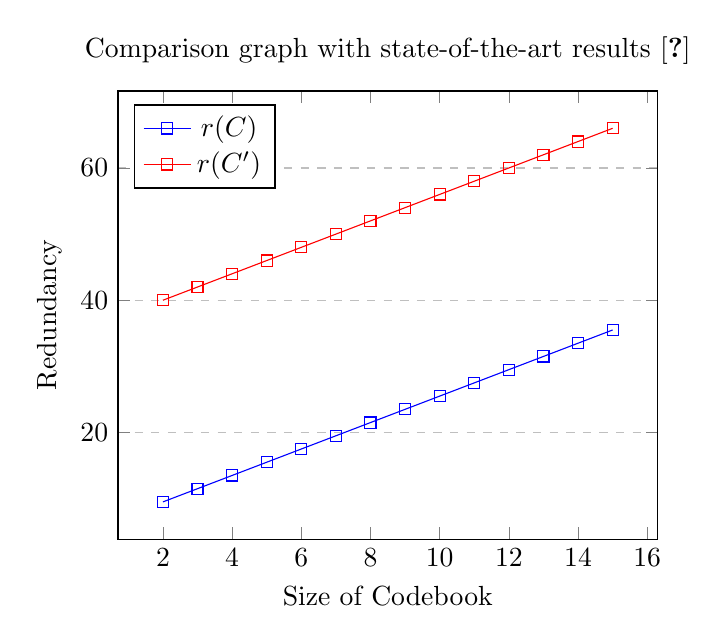
\begin{tikzpicture}
        \begin{axis}[
            title={Comparison graph with state-of-the-art results \cite{Smagloy_Welter_Wachter-Zeh_Yaakobi_2020}},
            xlabel={Size of Codebook},
            ylabel={Redundancy},
            legend pos=north west,
            ymajorgrids=true,
            grid style=dashed,
        ]
            \addplot[
                color=blue,
                mark=square,
                ]
                coordinates {
                    (2,9.5)(3,11.5)(4,13.5)(5,15.5)(6,17.5)(7,19.5)(8,21.5)(9,23.5)(10,25.5)(11,27.5)(12,29.5)(13,31.5)(14,33.5)(15,35.5)
                };
            \addlegendentry{$r(C)$}
            
            \addplot[
                color=red,
                mark=square,
                ]
                coordinates {
                    (2,40)(3,42)(4,44)(5,46)(6,48)(7,50)(8,52)(9,54)(10,56)(11,58)(12,60)(13,62)(14,64)(15,66)
                };
            \addlegendentry{$r(C')$}
        \end{axis}
    \end{tikzpicture}
    \caption{Our approach computes three times for different codebook sizes and returns the length of the sequence $n$. The state-of-the-art result is $10\log(n) + 3\log(q) + 11$, where $q=4$.}
\end{figure}

\end{document}